% Name: Transformer encoder layer
% Description: Multi-head attention and a feed-forward block, each with a residual connection and normalization, repeated N times.
% Tags: transformer, encoder, attention, residual connection

\usetikzlibrary{arrows.meta, positioning, fit, backgrounds}

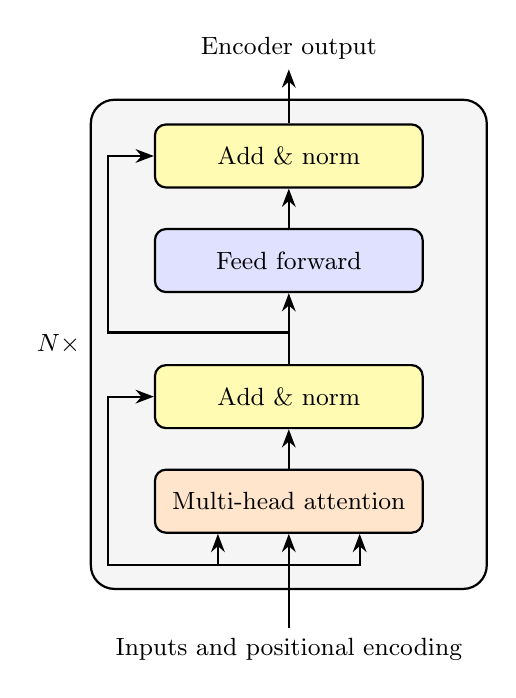
\begin{tikzpicture}[
  node distance=5mm,
  every node/.style={font=\small},
  sub/.style={draw, thick, rounded corners, minimum width=34mm, minimum height=8mm},
  arrow/.style={-{Stealth}, thick},
]
  \node[sub, fill=orange!20] (attn) {Multi-head attention};
  \node[sub, fill=yellow!30, above=of attn] (norm1) {Add \& norm};
  \node[sub, fill=blue!12, above=9mm of norm1] (ff) {Feed forward};
  \node[sub, fill=yellow!30, above=of ff] (norm2) {Add \& norm};
  \node[below=12mm of attn] (in) {Inputs and positional encoding};
  \coordinate[below=4mm of attn] (r1);
  \coordinate[above=4mm of norm1] (r2);

  \begin{scope}[on background layer]
    \node[draw, thick, rounded corners=3mm, fill=gray!8, fit=(attn)(norm2)(r1), inner xsep=8mm, inner ysep=3mm, label=left:{$N\times$}] {};
  \end{scope}

  \draw[arrow] (in) -- (attn);
  \foreach \dx in {-9mm, 9mm}
    \draw[arrow] (r1) -| ([xshift=\dx]attn.south);
  \draw[arrow] (r1) -- ++(-23mm,0) |- (norm1.west);
  \draw[arrow] (attn) -- (norm1);
  \draw[arrow] (norm1) -- (ff);
  \draw[arrow] (r2) -- ++(-23mm,0) |- (norm2.west);
  \draw[arrow] (ff) -- (norm2);
  \draw[arrow] (norm2) -- ++(0,11mm) node[above] {Encoder output};
\end{tikzpicture}
